\documentclass[12pt]{article}

%packages
%\usepackage{latexsym}
\usepackage{graphicx}
\usepackage{color}
\usepackage{amsmath}
\usepackage{dsfont}
\usepackage{placeins}
\usepackage{amssymb}
\usepackage{wasysym}
\usepackage{abstract}
\usepackage{hyperref}
\usepackage{etoolbox}
\usepackage{datetime}
\usepackage{xcolor}
\usepackage{alphalph}
\settimeformat{ampmtime}

%\usepackage{pstricks,pst-node,pst-tree}

%\usepackage{algpseudocode}
%\usepackage{amsthm}
%\usepackage{hyperref}
%\usepackage{mathrsfs}
%\usepackage{amsfonts}
%\usepackage{bbding}
%\usepackage{listings}
%\usepackage{appendix}
\usepackage[margin=1in]{geometry}
%\geometry{papersize={8.5in,11in},total={6.5in,9in}}
%\usepackage{cancel}
%\usepackage{algorithmic, algorithm}

\makeatletter
\def\maxwidth{ %
  \ifdim\Gin@nat@width>\linewidth
    \linewidth
  \else
    \Gin@nat@width
  \fi
}
\makeatother

\definecolor{fgcolor}{rgb}{0.345, 0.345, 0.345}
\newcommand{\hlnum}[1]{\textcolor[rgb]{0.686,0.059,0.569}{#1}}%
\newcommand{\hlstr}[1]{\textcolor[rgb]{0.192,0.494,0.8}{#1}}%
\newcommand{\hlcom}[1]{\textcolor[rgb]{0.678,0.584,0.686}{\textit{#1}}}%
\newcommand{\hlopt}[1]{\textcolor[rgb]{0,0,0}{#1}}%
\newcommand{\hlstd}[1]{\textcolor[rgb]{0.345,0.345,0.345}{#1}}%
\newcommand{\hlkwa}[1]{\textcolor[rgb]{0.161,0.373,0.58}{\textbf{#1}}}%
\newcommand{\hlkwb}[1]{\textcolor[rgb]{0.69,0.353,0.396}{#1}}%
\newcommand{\hlkwc}[1]{\textcolor[rgb]{0.333,0.667,0.333}{#1}}%
\newcommand{\hlkwd}[1]{\textcolor[rgb]{0.737,0.353,0.396}{\textbf{#1}}}%

\usepackage{framed}
\makeatletter
\newenvironment{kframe}{%
 \def\at@end@of@kframe{}%
 \ifinner\ifhmode%
  \def\at@end@of@kframe{\end{minipage}}%
  \begin{minipage}{\columnwidth}%
 \fi\fi%
 \def\FrameCommand##1{\hskip\@totalleftmargin \hskip-\fboxsep
 \colorbox{shadecolor}{##1}\hskip-\fboxsep
     % There is no \\@totalrightmargin, so:
     \hskip-\linewidth \hskip-\@totalleftmargin \hskip\columnwidth}%
 \MakeFramed {\advance\hsize-\width
   \@totalleftmargin\z@ \linewidth\hsize
   \@setminipage}}%
 {\par\unskip\endMakeFramed%
 \at@end@of@kframe}
\makeatother

\definecolor{shadecolor}{rgb}{.77, .77, .77}
\definecolor{messagecolor}{rgb}{0, 0, 0}
\definecolor{warningcolor}{rgb}{1, 0, 1}
\definecolor{errorcolor}{rgb}{1, 0, 0}
\newenvironment{knitrout}{}{} % an empty environment to be redefined in TeX

\usepackage{alltt}
\usepackage[T1]{fontenc}

\newcommand{\qu}[1]{``#1''}
\newcounter{probnum}
\setcounter{probnum}{1}

%create definition to allow local margin changes
\def\changemargin#1#2{\list{}{\rightmargin#2\leftmargin#1}\item[]}
\let\endchangemargin=\endlist 

%allow equations to span multiple pages
\allowdisplaybreaks

%define colors and color typesetting conveniences
\definecolor{gray}{rgb}{0.5,0.5,0.5}
\definecolor{black}{rgb}{0,0,0}
\definecolor{white}{rgb}{1,1,1}
\definecolor{blue}{rgb}{0.5,0.5,1}
\newcommand{\inblue}[1]{\color{blue}#1 \color{black}}
\definecolor{green}{rgb}{0.133,0.545,0.133}
\newcommand{\ingreen}[1]{\color{green}#1 \color{black}}
\definecolor{yellow}{rgb}{1,1,0}
\newcommand{\inyellow}[1]{\color{yellow}#1 \color{black}}
\definecolor{orange}{rgb}{0.9,0.649,0}
\newcommand{\inorange}[1]{\color{orange}#1 \color{black}}
\definecolor{red}{rgb}{1,0.133,0.133}
\newcommand{\inred}[1]{\color{red}#1 \color{black}}
\definecolor{purple}{rgb}{0.58,0,0.827}
\newcommand{\inpurple}[1]{\color{purple}#1 \color{black}}
\definecolor{backgcode}{rgb}{0.97,0.97,0.8}
\definecolor{Brown}{cmyk}{0,0.81,1,0.60}
\definecolor{OliveGreen}{cmyk}{0.64,0,0.95,0.40}
\definecolor{CadetBlue}{cmyk}{0.62,0.57,0.23,0}

%define new math operators
\DeclareMathOperator*{\argmax}{arg\,max~}
\DeclareMathOperator*{\argmin}{arg\,min~}
\DeclareMathOperator*{\argsup}{arg\,sup~}
\DeclareMathOperator*{\arginf}{arg\,inf~}
\DeclareMathOperator*{\convolution}{\text{\Huge{$\ast$}}}
\newcommand{\infconv}[2]{\convolution^\infty_{#1 = 1} #2}
%true functions

%%%% GENERAL SHORTCUTS

%shortcuts for pure typesetting conveniences
\newcommand{\bv}[1]{\boldsymbol{#1}}

%shortcuts for compound constants
\newcommand{\BetaDistrConst}{\dfrac{\Gamma(\alpha + \beta)}{\Gamma(\alpha)\Gamma(\beta)}}
\newcommand{\NormDistrConst}{\dfrac{1}{\sqrt{2\pi\sigma^2}}}

%shortcuts for conventional symbols
\newcommand{\tsq}{\tau^2}
\newcommand{\tsqh}{\hat{\tau}^2}
\newcommand{\sigsq}{\sigma^2}
\newcommand{\sigsqsq}{\parens{\sigma^2}^2}
\newcommand{\sigsqovern}{\dfrac{\sigsq}{n}}
\newcommand{\tausq}{\tau^2}
\newcommand{\tausqalpha}{\tau^2_\alpha}
\newcommand{\tausqbeta}{\tau^2_\beta}
\newcommand{\tausqsigma}{\tau^2_\sigma}
\newcommand{\betasq}{\beta^2}
\newcommand{\sigsqvec}{\bv{\sigma}^2}
\newcommand{\sigsqhat}{\hat{\sigma}^2}
\newcommand{\sigsqhatmlebayes}{\sigsqhat_{\text{Bayes, MLE}}}
\newcommand{\sigsqhatmle}[1]{\sigsqhat_{#1, \text{MLE}}}
\newcommand{\bSigma}{\bv{\Sigma}}
\newcommand{\bSigmainv}{\bSigma^{-1}}
\newcommand{\thetavec}{\bv{\theta}}
\newcommand{\thetahat}{\hat{\theta}}
\newcommand{\thetahatmle}{\hat{\theta}_{\mathrm{MLE}}}
\newcommand{\thetavechatmle}{\hat{\thetavec}_{\mathrm{MLE}}}
\newcommand{\muhat}{\hat{\mu}}
\newcommand{\musq}{\mu^2}
\newcommand{\muvec}{\bv{\mu}}
\newcommand{\muhatmle}{\muhat_{\text{MLE}}}
\newcommand{\lambdahat}{\hat{\lambda}}
\newcommand{\lambdahatmle}{\lambdahat_{\text{MLE}}}
\newcommand{\etavec}{\bv{\eta}}
\newcommand{\alphavec}{\bv{\alpha}}
\newcommand{\minimaxdec}{\delta^*_{\mathrm{mm}}}
\newcommand{\ybar}{\bar{y}}
\newcommand{\xbar}{\bar{x}}
\newcommand{\Xbar}{\bar{X}}
\newcommand{\phat}{\hat{p}}
\newcommand{\Phat}{\hat{P}}
\newcommand{\Zbar}{\bar{Z}}
\newcommand{\iid}{~{\buildrel iid \over \sim}~}
\newcommand{\inddist}{~{\buildrel ind \over \sim}~}
\newcommand{\approxdist}{~{\buildrel approx \over \sim}~}
\newcommand{\equalsindist}{~{\buildrel d \over =}~}
\newcommand{\loglik}[1]{\ell\parens{#1}}
\newcommand{\thetahatkminone}{\thetahat^{(k-1)}}
\newcommand{\thetahatkplusone}{\thetahat^{(k+1)}}
\newcommand{\thetahatk}{\thetahat^{(k)}}
\newcommand{\half}{\frac{1}{2}}
\newcommand{\third}{\frac{1}{3}}
\newcommand{\twothirds}{\frac{2}{3}}
\newcommand{\fourth}{\frac{1}{4}}
\newcommand{\fifth}{\frac{1}{5}}
\newcommand{\sixth}{\frac{1}{6}}

%shortcuts for vector and matrix notation
\newcommand{\A}{\bv{A}}
\renewcommand{\b}{\bv{b}}
\newcommand{\w}{\bv{w}}
\newcommand{\At}{\A^T}
\newcommand{\Ainv}{\inverse{\A}}
\newcommand{\B}{\bv{B}}
\newcommand{\K}{\bv{K}}
\newcommand{\Kt}{\K^T}
\newcommand{\Kinv}{\inverse{K}}
\newcommand{\Kinvt}{(\Kinv)^T}
\newcommand{\M}{\bv{M}}
\newcommand{\Bt}{\B^T}
\newcommand{\Q}{\bv{Q}}
\newcommand{\Qt}{\Q^T}
\newcommand{\R}{\bv{R}}
\newcommand{\Rt}{\R^T}
\newcommand{\Z}{\bv{Z}}
\newcommand{\X}{\bv{X}}
\newcommand{\Xsub}{\X_{\text{(sub)}}}
\newcommand{\Xsubadj}{\X_{\text{(sub,adj)}}}
\newcommand{\I}{\bv{I}}
\newcommand{\Y}{\bv{Y}}
\newcommand{\sigsqI}{\sigsq\I}
\renewcommand{\P}{\bv{P}}
\newcommand{\Psub}{\P_{\text{(sub)}}}
\newcommand{\Pt}{\P^T}
\newcommand{\Pii}{P_{ii}}
\newcommand{\Pij}{P_{ij}}
\newcommand{\IminP}{(\I-\P)}
\newcommand{\Xt}{X^\top}
\newcommand{\XtX}{\Xt X}
\newcommand{\XtXinv}{\parens{\Xt X}^{-1}}
\newcommand{\XtXinvXt}{\XtXinv\Xt}
\newcommand{\XXtXinvXt}{X\XtXinvXt}
\newcommand{\x}{\bv{x}}
\newcommand{\onevec}{\bv{1}}
\newcommand{\zerovec}{\bv{0}}
\newcommand{\oneton}{1, \ldots, n}
\newcommand{\yoneton}{y_1, \ldots, y_n}
\newcommand{\yonetonorder}{y_{(1)}, \ldots, y_{(n)}}
\newcommand{\Yoneton}{Y_1, \ldots, Y_n}
\newcommand{\iinoneton}{i \in \braces{\oneton}}
\newcommand{\onetom}{1, \ldots, m}
\newcommand{\jinonetom}{j \in \braces{\onetom}}
\newcommand{\xoneton}{x_1, \ldots, x_n}
\newcommand{\Xoneton}{X_1, \ldots, X_n}
\newcommand{\xt}{\x^T}
\newcommand{\y}{\bv{y}}
\newcommand{\yt}{\y^T}
\renewcommand{\c}{\bv{c}}
\newcommand{\ct}{\c^T}
\newcommand{\tstar}{\bv{t}^*}
\renewcommand{\u}{\bv{u}}
\renewcommand{\v}{\bv{v}}
\renewcommand{\a}{\bv{a}}
\newcommand{\s}{\bv{s}}
\newcommand{\yadj}{\y_{\text{(adj)}}}
\newcommand{\xjadj}{\x_{j\text{(adj)}}}
\newcommand{\xjadjM}{\x_{j \perp M}}
\newcommand{\yhat}{\hat{\y}}
\newcommand{\yhatsub}{\yhat_{\text{(sub)}}}
\newcommand{\yhatstar}{\yhat^*}
\newcommand{\yhatstarnew}{\yhatstar_{\text{new}}}
\newcommand{\z}{\bv{z}}
\newcommand{\zt}{\z^T}
\newcommand{\bb}{\bv{b}}
\newcommand{\bbt}{\bb^T}
\newcommand{\bbeta}{\bv{\beta}}
\newcommand{\beps}{\bv{\epsilon}}
\newcommand{\bepst}{\beps^T}
\newcommand{\e}{\bv{e}}
\newcommand{\Mofy}{\M(\y)}
\newcommand{\KofAlpha}{K(\alpha)}
\newcommand{\ellset}{\mathcal{L}}
\newcommand{\oneminalph}{1-\alpha}
\newcommand{\SSE}{\text{SSE}}
\newcommand{\SSEsub}{\text{SSE}_{\text{(sub)}}}
\newcommand{\MSE}{\text{MSE}}
\newcommand{\RMSE}{\text{RMSE}}
\newcommand{\SSR}{\text{SSR}}
\newcommand{\SST}{\text{SST}}
\newcommand{\JSest}{\delta_{\text{JS}}(\x)}
\newcommand{\Bayesest}{\delta_{\text{Bayes}}(\x)}
\newcommand{\EmpBayesest}{\delta_{\text{EmpBayes}}(\x)}
\newcommand{\BLUPest}{\delta_{\text{BLUP}}}
\newcommand{\MLEest}[1]{\hat{#1}_{\text{MLE}}}

%shortcuts for Linear Algebra stuff (i.e. vectors and matrices)
\newcommand{\twovec}[2]{\bracks{\begin{array}{c} #1 \\ #2 \end{array}}}
\newcommand{\threevec}[3]{\bracks{\begin{array}{c} #1 \\ #2 \\ #3 \end{array}}}
\newcommand{\fivevec}[5]{\bracks{\begin{array}{c} #1 \\ #2 \\ #3 \\ #4 \\ #5 \end{array}}}
\newcommand{\twobytwomat}[4]{\bracks{\begin{array}{cc} #1 & #2 \\ #3 & #4 \end{array}}}
\newcommand{\threebytwomat}[6]{\bracks{\begin{array}{cc} #1 & #2 \\ #3 & #4 \\ #5 & #6 \end{array}}}


%shortcuts for conventional compound symbols
\newcommand{\thetainthetas}{\theta \in \Theta}
\newcommand{\reals}{\mathbb{R}}
\newcommand{\complexes}{\mathbb{C}}
\newcommand{\rationals}{\mathbb{Q}}
\newcommand{\integers}{\mathbb{Z}}
\newcommand{\naturals}{\mathbb{N}}
\newcommand{\forallninN}{~~\forall n \in \naturals}
\newcommand{\forallxinN}[1]{~~\forall #1 \in \reals}
\newcommand{\matrixdims}[2]{\in \reals^{\,#1 \times #2}}
\newcommand{\inRn}[1]{\in \reals^{\,#1}}
\newcommand{\mathimplies}{\quad\Rightarrow\quad}
\newcommand{\mathlogicequiv}{\quad\Leftrightarrow\quad}
\newcommand{\eqncomment}[1]{\quad \text{(#1)}}
\newcommand{\limitn}{\lim_{n \rightarrow \infty}}
\newcommand{\limitN}{\lim_{N \rightarrow \infty}}
\newcommand{\limitd}{\lim_{d \rightarrow \infty}}
\newcommand{\limitt}{\lim_{t \rightarrow \infty}}
\newcommand{\limitsupn}{\limsup_{n \rightarrow \infty}~}
\newcommand{\limitinfn}{\liminf_{n \rightarrow \infty}~}
\newcommand{\limitk}{\lim_{k \rightarrow \infty}}
\newcommand{\limsupn}{\limsup_{n \rightarrow \infty}}
\newcommand{\limsupk}{\limsup_{k \rightarrow \infty}}
\newcommand{\floor}[1]{\left\lfloor #1 \right\rfloor}
\newcommand{\ceil}[1]{\left\lceil #1 \right\rceil}

%shortcuts for environments
\newcommand{\beqn}{\vspace{-0.25cm}\begin{eqnarray*}}
\newcommand{\eeqn}{\end{eqnarray*}}
\newcommand{\bneqn}{\vspace{-0.25cm}\begin{eqnarray}}
\newcommand{\eneqn}{\end{eqnarray}}

%shortcuts for mini environments
\newcommand{\parens}[1]{\left(#1\right)}
\newcommand{\squared}[1]{\parens{#1}^2}
\newcommand{\tothepow}[2]{\parens{#1}^{#2}}
\newcommand{\prob}[1]{\mathbb{P}\parens{#1}}
\newcommand{\cprob}[2]{\prob{#1~|~#2}}
\newcommand{\littleo}[1]{o\parens{#1}}
\newcommand{\bigo}[1]{O\parens{#1}}
\newcommand{\Lp}[1]{\mathbb{L}^{#1}}
\renewcommand{\arcsin}[1]{\text{arcsin}\parens{#1}}
\newcommand{\prodonen}[2]{\bracks{\prod_{#1=1}^n #2}}
\newcommand{\mysum}[4]{\sum_{#1=#2}^{#3} #4}
\newcommand{\sumonen}[2]{\sum_{#1=1}^n #2}
\newcommand{\infsum}[2]{\sum_{#1=1}^\infty #2}
\newcommand{\infprod}[2]{\prod_{#1=1}^\infty #2}
\newcommand{\infunion}[2]{\bigcup_{#1=1}^\infty #2}
\newcommand{\infinter}[2]{\bigcap_{#1=1}^\infty #2}
\newcommand{\infintegral}[2]{\int^\infty_{-\infty} #2 ~\text{d}#1}
\newcommand{\supthetas}[1]{\sup_{\thetainthetas}\braces{#1}}
\newcommand{\bracks}[1]{\left[#1\right]}
\newcommand{\braces}[1]{\left\{#1\right\}}
\newcommand{\set}[1]{\left\{#1\right\}}
\newcommand{\abss}[1]{\left|#1\right|}
\newcommand{\norm}[1]{\left|\left|#1\right|\right|}
\newcommand{\normsq}[1]{\norm{#1}^2}
\newcommand{\inverse}[1]{\parens{#1}^{-1}}
\newcommand{\rowof}[2]{\parens{#1}_{#2\cdot}}

%shortcuts for functionals
\newcommand{\realcomp}[1]{\text{Re}\bracks{#1}}
\newcommand{\imagcomp}[1]{\text{Im}\bracks{#1}}
\newcommand{\range}[1]{\text{range}\bracks{#1}}
\newcommand{\colsp}[1]{\text{colsp}\bracks{#1}}
\newcommand{\rowsp}[1]{\text{rowsp}\bracks{#1}}
\newcommand{\tr}[1]{\text{tr}\bracks{#1}}
\newcommand{\rank}[1]{\text{rank}\bracks{#1}}
\newcommand{\proj}[2]{\text{Proj}_{#1}\bracks{#2}}
\newcommand{\projcolspX}[1]{\text{Proj}_{\colsp{\X}}\bracks{#1}}
\newcommand{\median}[1]{\text{median}\bracks{#1}}
\newcommand{\mean}[1]{\text{mean}\bracks{#1}}
\newcommand{\dime}[1]{\text{dim}\bracks{#1}}
\renewcommand{\det}[1]{\text{det}\bracks{#1}}
\newcommand{\expe}[1]{\mathbb{E}\bracks{#1}}
\newcommand{\expeabs}[1]{\expe{\abss{#1}}}
\newcommand{\expesub}[2]{\mathbb{E}_{#1}\bracks{#2}}
\newcommand{\indic}[1]{\mathds{1}_{#1}}
\newcommand{\var}[1]{\mathbb{V}\text{ar}\bracks{#1}}
\newcommand{\cov}[2]{\mathbb{C}\text{ov}\bracks{#1, #2}}
\newcommand{\corr}[2]{\text{Corr}\bracks{#1, #2}}
\newcommand{\se}[1]{\mathbb{S}\text{E}\bracks{#1}}
\newcommand{\seest}[1]{\hat{\mathbb{S}\text{E}}\bracks{#1}}
\newcommand{\bias}[1]{\text{Bias}\bracks{#1}}
\newcommand{\derivop}[2]{\dfrac{\text{d}}{\text{d} #1}\bracks{#2}}
\newcommand{\partialop}[2]{\dfrac{\partial}{\partial #1}\bracks{#2}}
\newcommand{\secpartialop}[2]{\dfrac{\partial^2}{\partial #1^2}\bracks{#2}}
\newcommand{\mixpartialop}[3]{\dfrac{\partial^2}{\partial #1 \partial #2}\bracks{#3}}

%shortcuts for functions
\renewcommand{\exp}[1]{\mathrm{exp}\parens{#1}}
\renewcommand{\cos}[1]{\text{cos}\parens{#1}}
\renewcommand{\sin}[1]{\text{sin}\parens{#1}}
\newcommand{\sign}[1]{\text{sign}\parens{#1}}
\newcommand{\are}[1]{\mathrm{ARE}\parens{#1}}
\newcommand{\natlog}[1]{\ln\parens{#1}}
\newcommand{\oneover}[1]{\frac{1}{#1}}
\newcommand{\overtwo}[1]{\frac{#1}{2}}
\newcommand{\overn}[1]{\frac{#1}{n}}
\newcommand{\oneoversqrt}[1]{\oneover{\sqrt{#1}}}
\newcommand{\sqd}[1]{\parens{#1}^2}
\newcommand{\loss}[1]{\ell\parens{\theta, #1}}
\newcommand{\losstwo}[2]{\ell\parens{#1, #2}}
\newcommand{\cf}{\phi(t)}

%English language specific shortcuts
\newcommand{\ie}{\textit{i.e.} }
\newcommand{\AKA}{\textit{AKA} }
\renewcommand{\iff}{\textit{iff}}
\newcommand{\eg}{\textit{e.g.} }
\newcommand{\st}{\textit{s.t.} }
\newcommand{\wrt}{\textit{w.r.t.} }
\newcommand{\mathst}{~~\text{\st}~~}
\newcommand{\mathand}{~~\text{and}~~}
\newcommand{\ala}{\textit{a la} }
\newcommand{\ppp}{posterior predictive p-value}
\newcommand{\dd}{dataset-to-dataset}

%shortcuts for distribution titles
\newcommand{\logistic}[2]{\mathrm{Logistic}\parens{#1,\,#2}}
\newcommand{\bernoulli}[1]{\mathrm{Bernoulli}\parens{#1}}
\newcommand{\betanot}[2]{\mathrm{Beta}\parens{#1,\,#2}}
\newcommand{\stdbetanot}{\betanot{\alpha}{\beta}}
\newcommand{\multnormnot}[3]{\mathcal{N}_{#1}\parens{#2,\,#3}}
\newcommand{\normnot}[2]{\mathcal{N}\parens{#1,\,#2}}
\newcommand{\classicnormnot}{\normnot{\mu}{\sigsq}}
\newcommand{\stdnormnot}{\normnot{0}{1}}
\newcommand{\uniformdiscrete}[1]{\mathrm{Uniform}\parens{\braces{#1}}}
\newcommand{\uniform}[2]{\mathrm{U}\parens{#1,\,#2}}
\newcommand{\stduniform}{\uniform{0}{1}}
\newcommand{\geometric}[1]{\mathrm{Geometric}\parens{#1}}
\newcommand{\hypergeometric}[3]{\mathrm{Hypergeometric}\parens{#1,\,#2,\,#3}}
\newcommand{\exponential}[1]{\mathrm{Exp}\parens{#1}}
\newcommand{\gammadist}[2]{\mathrm{Gamma}\parens{#1, #2}}
\newcommand{\poisson}[1]{\mathrm{Poisson}\parens{#1}}
\newcommand{\binomial}[2]{\mathrm{Binomial}\parens{#1,\,#2}}
\newcommand{\negbin}[2]{\mathrm{NegBin}\parens{#1,\,#2}}
\newcommand{\rayleigh}[1]{\mathrm{Rayleigh}\parens{#1}}
\newcommand{\multinomial}[2]{\mathrm{Multinomial}\parens{#1,\,#2}}
\newcommand{\gammanot}[2]{\mathrm{Gamma}\parens{#1,\,#2}}
\newcommand{\cauchynot}[2]{\text{Cauchy}\parens{#1,\,#2}}
\newcommand{\invchisqnot}[1]{\text{Inv}\chisq{#1}}
\newcommand{\invscaledchisqnot}[2]{\text{ScaledInv}\ncchisq{#1}{#2}}
\newcommand{\invgammanot}[2]{\text{InvGamma}\parens{#1,\,#2}}
\newcommand{\chisq}[1]{\chi^2_{#1}}
\newcommand{\ncchisq}[2]{\chi^2_{#1}\parens{#2}}
\newcommand{\ncF}[3]{F_{#1,#2}\parens{#3}}

%shortcuts for PDF's of common distributions
\newcommand{\logisticpdf}[3]{\oneover{#3}\dfrac{\exp{-\dfrac{#1 - #2}{#3}}}{\parens{1+\exp{-\dfrac{#1 - #2}{#3}}}^2}}
\newcommand{\betapdf}[3]{\dfrac{\Gamma(#2 + #3)}{\Gamma(#2)\Gamma(#3)}#1^{#2-1} (1-#1)^{#3-1}}
\newcommand{\normpdf}[3]{\frac{1}{\sqrt{2\pi#3}}\exp{-\frac{1}{2#3}(#1 - #2)^2}}
\newcommand{\normpdfvarone}[2]{\dfrac{1}{\sqrt{2\pi}}e^{-\half(#1 - #2)^2}}
\newcommand{\chisqpdf}[2]{\dfrac{1}{2^{#2/2}\Gamma(#2/2)}\; {#1}^{#2/2-1} e^{-#1/2}}
\newcommand{\invchisqpdf}[2]{\dfrac{2^{-\overtwo{#1}}}{\Gamma(#2/2)}\,{#1}^{-\overtwo{#2}-1}  e^{-\oneover{2 #1}}}
\newcommand{\exponentialpdf}[2]{#2\exp{-#2#1}}
\newcommand{\poissonpdf}[2]{\dfrac{e^{-#1} #1^{#2}}{#2!}}
\newcommand{\binomialpdf}[3]{\binom{#2}{#1}#3^{#1}(1-#3)^{#2-#1}}
\newcommand{\rayleighpdf}[2]{\dfrac{#1}{#2^2}\exp{-\dfrac{#1^2}{2 #2^2}}}
\newcommand{\gammapdf}[3]{\dfrac{#3^#2}{\Gamma\parens{#2}}#1^{#2-1}\exp{-#3 #1}}
\newcommand{\cauchypdf}[3]{\oneover{\pi} \dfrac{#3}{\parens{#1-#2}^2 + #3^2}}
\newcommand{\Gammaf}[1]{\Gamma\parens{#1}}

%shortcuts for miscellaneous typesetting conveniences
\newcommand{\notesref}[1]{\marginpar{\color{gray}\tt #1\color{black}}}

%%%% DOMAIN-SPECIFIC SHORTCUTS

%Real analysis related shortcuts
\newcommand{\zeroonecl}{\bracks{0,1}}
\newcommand{\forallepsgrzero}{\forall \epsilon > 0~~}
\newcommand{\lessthaneps}{< \epsilon}
\newcommand{\fraccomp}[1]{\text{frac}\bracks{#1}}

%Bayesian related shortcuts
\newcommand{\yrep}{y^{\text{rep}}}
\newcommand{\yrepisq}{(\yrep_i)^2}
\newcommand{\yrepvec}{\bv{y}^{\text{rep}}}


%Probability shortcuts
\newcommand{\SigField}{\mathcal{F}}
\newcommand{\ProbMap}{\mathcal{P}}
\newcommand{\probtrinity}{\parens{\Omega, \SigField, \ProbMap}}
\newcommand{\convp}{~{\buildrel p \over \rightarrow}~}
\newcommand{\convLp}[1]{~{\buildrel \Lp{#1} \over \rightarrow}~}
\newcommand{\nconvp}{~{\buildrel p \over \nrightarrow}~}
\newcommand{\convae}{~{\buildrel a.e. \over \longrightarrow}~}
\newcommand{\convau}{~{\buildrel a.u. \over \longrightarrow}~}
\newcommand{\nconvau}{~{\buildrel a.u. \over \nrightarrow}~}
\newcommand{\nconvae}{~{\buildrel a.e. \over \nrightarrow}~}
\newcommand{\convd}{~{\buildrel \mathcal{D} \over \rightarrow}~}
\newcommand{\nconvd}{~{\buildrel \mathcal{D} \over \nrightarrow}~}
\newcommand{\withprob}{~~\text{w.p.}~~}
\newcommand{\io}{~~\text{i.o.}}

\newcommand{\Acl}{\bar{A}}
\newcommand{\ENcl}{\bar{E}_N}
\newcommand{\diam}[1]{\text{diam}\parens{#1}}

\newcommand{\taua}{\tau_a}

\newcommand{\myint}[4]{\int_{#2}^{#3} #4 \,\text{d}#1}
\newcommand{\laplacet}[1]{\mathscr{L}\bracks{#1}}
\newcommand{\laplaceinvt}[1]{\mathscr{L}^{-1}\bracks{#1}}
\renewcommand{\min}[1]{\text{min}\braces{#1}}
\renewcommand{\max}[1]{\text{max}\braces{#1}}

\newcommand{\Vbar}[1]{\bar{V}\parens{#1}}
\newcommand{\expnegrtau}{\exp{-r\tau}}

%%% problem typesetting
\definecolor{darkgrey}{rgb}{0.10,0.10,0.9}

\newcommand{\problem}[1]{\noindent \colorbox{black}{{\color{yellow} \large{\textsf{\textbf{Problem \arabic{probnum}}}}~}} \addtocounter{probnum}{1} \vspace{0.2cm} \\ \iftoggle{professormode}{}{\color{darkgrey}} #1}

\newcommand{\easysubproblem}[1]{\ingreen{\item} \iftoggle{professormode}{}{\color{darkgrey}} [easy] #1 \color{black} }
\newcommand{\intermediatesubproblem}[1]{\inorange{\item} \iftoggle{professormode}{}{\color{darkgrey}} [harder] #1 \color{black} }
\newcommand{\hardsubproblem}[1]{\inred{\item} \iftoggle{professormode}{}{\color{darkgrey}} [difficult] #1 \color{black} }
\newcommand{\extracreditsubproblem}[1]{\inpurple{\item} \iftoggle{professormode}{}{\color{darkgrey}} [E.C.] #1 \color{black} }


\newcommand{\spc}[1]{\iftoggle{professormode}{\\ \vspace{#1cm}}{\\ \vspace{-0.3cm}}}

\makeatletter
\newalphalph{\alphmult}[mult]{\@alph}{26}
\renewcommand{\labelenumi}{(\alphmult{\value{enumi}})}

\newcommand{\support}[1]{\text{Supp}\bracks{#1}}
\newcommand{\mode}[1]{\text{Mode}\bracks{#1}}
\newcommand{\IQR}[1]{\text{IQR}\bracks{#1}}
\newcommand{\quantile}[2]{\text{Quantile}\bracks{#1,\,#2}}


\newtoggle{professormode}
%\toggletrue{professormode} %STUDENTS: DELETE or COMMENT this line



\title{MATH 390.4 / 650.2 Spring 2018 Homework \#1t}

\author{Rebecca Strauss} %STUDENTS: write your name here

\iftoggle{professormode}{
\date{Due \emph{in class} Monday, February 26, 2018 \\ \vspace{0.5cm} \small (this document last updated \today ~at \currenttime)}
}



\begin{document}
\maketitle

\iftoggle{professormode}{
\begin{abstract}
The path to success in this class is to do many problems. Unlike other courses, exclusively doing reading(s) will not help. Coming to lecture is akin to watching workout videos; thinking about and solving problems on your own is the actual ``working out.''  Feel free to \qu{work out} with others; \textbf{I want you to work on this in groups.}

Reading is still \textit{required}. For this homework set, read the first chapter of \qu{Learning from Data}. Also, read about all the concepts introduced in class online. This is your responsibility to supplement in-class with your own readings.

The problems below are color coded: \ingreen{green} problems are considered \textit{easy} and marked \qu{[easy]}; \inorange{yellow} problems are considered \textit{intermediate} and marked \qu{[harder]}, \inred{red} problems are considered \textit{difficult} and marked \qu{[difficult]} and \inpurple{purple} problems are extra credit. The \textit{easy} problems are intended to be ``giveaways'' if you went to class. Do as much as you can of the others; I expect you to at least attempt the \textit{difficult} problems. 

This homework is worth 100 points but the point distribution will not be determined until after the due date. See syllabus for the policy on late homework.

Up to 10 points are given as a bonus if the homework is typed using \LaTeX. Links to instaling \LaTeX~and program for compiling \LaTeX~is found on the syllabus. You are encouraged to use \url{overleaf.com}. If you are handing in homework this way, read the comments in the code; there are two lines to comment out and you should replace my name with yours and write your section. The easiest way to use overleaf is to copy the raw text from hwxx.tex and preamble.tex into two new overleaf tex files with the same name. If you are asked to make drawings, you can take a picture of your handwritten drawing and insert them as figures or leave space using the \qu{$\backslash$vspace} command and draw them in after printing or attach them stapled.

The document is available with spaces for you to write your answers. If not using \LaTeX, print this document and write in your answers. I do not accept homeworks which are \textit{not} on this printout. Keep this first page printed for your records.

\end{abstract}

\thispagestyle{empty}
\vspace{1cm}
NAME: \line(1,0){380}
\clearpage
}

\problem{These are questions about Silver's book, the introduction and chapter 1.}

\begin{enumerate}

\easysubproblem{What is the difference between \emph{predict} and \emph{forecast}? Are these two terms used interchangeably today?}\spc{4}

Although terms 'predict' and  'forecast' are used interchangeably today, in earlier centuries, the two were not synonymous. Predictions were associated with fortune telling and other whimsical practices. Forecasting involved using knowledge to plan ahead for the future.

\easysubproblem{What is John P. Ioannidis's findings and what are its implications?}\spc{5}

John P. Ioannidis's found that most experiments conducting in a laboratory setting, would fail if recreated in the real world. This implies that there is something fundamentally wrong with the way that "certified" scientists run their experiments and/or interpret results.

\easysubproblem{What are the human being's most powerful defense (according to Silver)? Answer using the language from class.}\spc{4}

Human being's most power defense is our mind, according to Silver. As humans, we have the ability to notice patterns in the world around us.

\easysubproblem{Information is increasing at a rapid pace, but what is not increasing?}\spc{3}

The amount of useful information is not increasing.

\hardsubproblem{Silver admits that we will always be subjectively biased when making predictions. However, he believes there is an objective truth. In class, how did we describe the objective truth? Answer using notation from class i.e. $t,f, g, h^*, \delta, \epsilon, t, z_1, \ldots, z_t, \delta, \mathbb{D}$, $\mathcal{H}, \mathcal{A}, \mathcal{X}, \mathcal{Y}, X, y, n, p$, $x_{\cdot 1}, \ldots, x_{\cdot p}, x_{1 \cdot}, \ldots, x_{n \cdot}$, etc.}\spc{3}
\begin{equation*}
y=t(z_1,\cdots , z_t)
\end{equation*}

\easysubproblem{In a nutshell, what is Karl Popper's (a famous philosopher of science) definition of \emph{science}?}\spc{4}

Science is anything that can be tested in the real world with predictions. 

\intermediatesubproblem{Why did the ratings agencies say the probability of a CDO defaulting was 0.12\% instead of the 28\% that actually occured? Answer using concepts from class.}\spc{4}

They made the wrong assumptions. They assumed that an individual defaulting on his mortgage is uncorrelated to others defaulting on their loan. The combination of the housing bubble burst and a bad economy created a common factor among mortgage holders and made them all more likely to default. Additionally, the error in the CDO models were nonlinear, making the error compound very quickly once a mistake was made.

\easysubproblem{What is the difference between \emph{risk} and \emph{uncertainty} according to Silver's definitions?}\spc{4}

Risk is something you can calculate and assign a number or probability to. Uncertainty is unquantifiable. 

\hardsubproblem{How does Silver define \emph{out of sample}? Answer using notation from class i.e. $t,f, g, h^*, \delta, \epsilon, t, z_1, \ldots, z_t, \delta, \mathbb{D}, \mathcal{H}, \mathcal{A}, \mathcal{X}, \mathcal{Y}, X, y, n, p, x_{\cdot 1}, \ldots, x_{\cdot p}, x_{1 \cdot}, \ldots, x_{n \cdot}$, etc. WARNING: Silver defines \emph{out of sample} completely differently than the literature (and differently than practitioners in industry). We will explore what he is talking about in class in the future and we will term this concept differently, using the more widely accepted terminology. So please forget the phrase \emph{out of sample} for now as we will introduce it later in class as something else. There will be other such terms in his book and I will provide this disclaimer at these appropriate times.}\spc{7}

Silver defines out of sample as an event that is not included in your historical data set.
\begin{equation*}
\mathcal{X}\not\subset\mathbb{D} 
\end{equation*}

\intermediatesubproblem{Look up \emph{bias} and \emph{variance} online or in a statistics textbook. Connect these concepts to Silver's terms \emph{accuracy} and \emph{precision}. This is another example of Silver using non-standard terminology.}\spc{6}

\end{enumerate}


\problem{Below are some questions about the theory of modeling.}

\begin{enumerate}

\easysubproblem{Redraw the illustration from lecture one except do not use the Earth and a table-top globe. In the top right quadrant, you should write \qu{predictions} not \qu{data} (this was my mistake in the notes). \qu{Data / measurements} are reserved for the bottom right quadrant. The quadrants are connected with arrows. Label these arrows appropriately as well..}\spc{12}

\begin{figure}[htp]
\centering
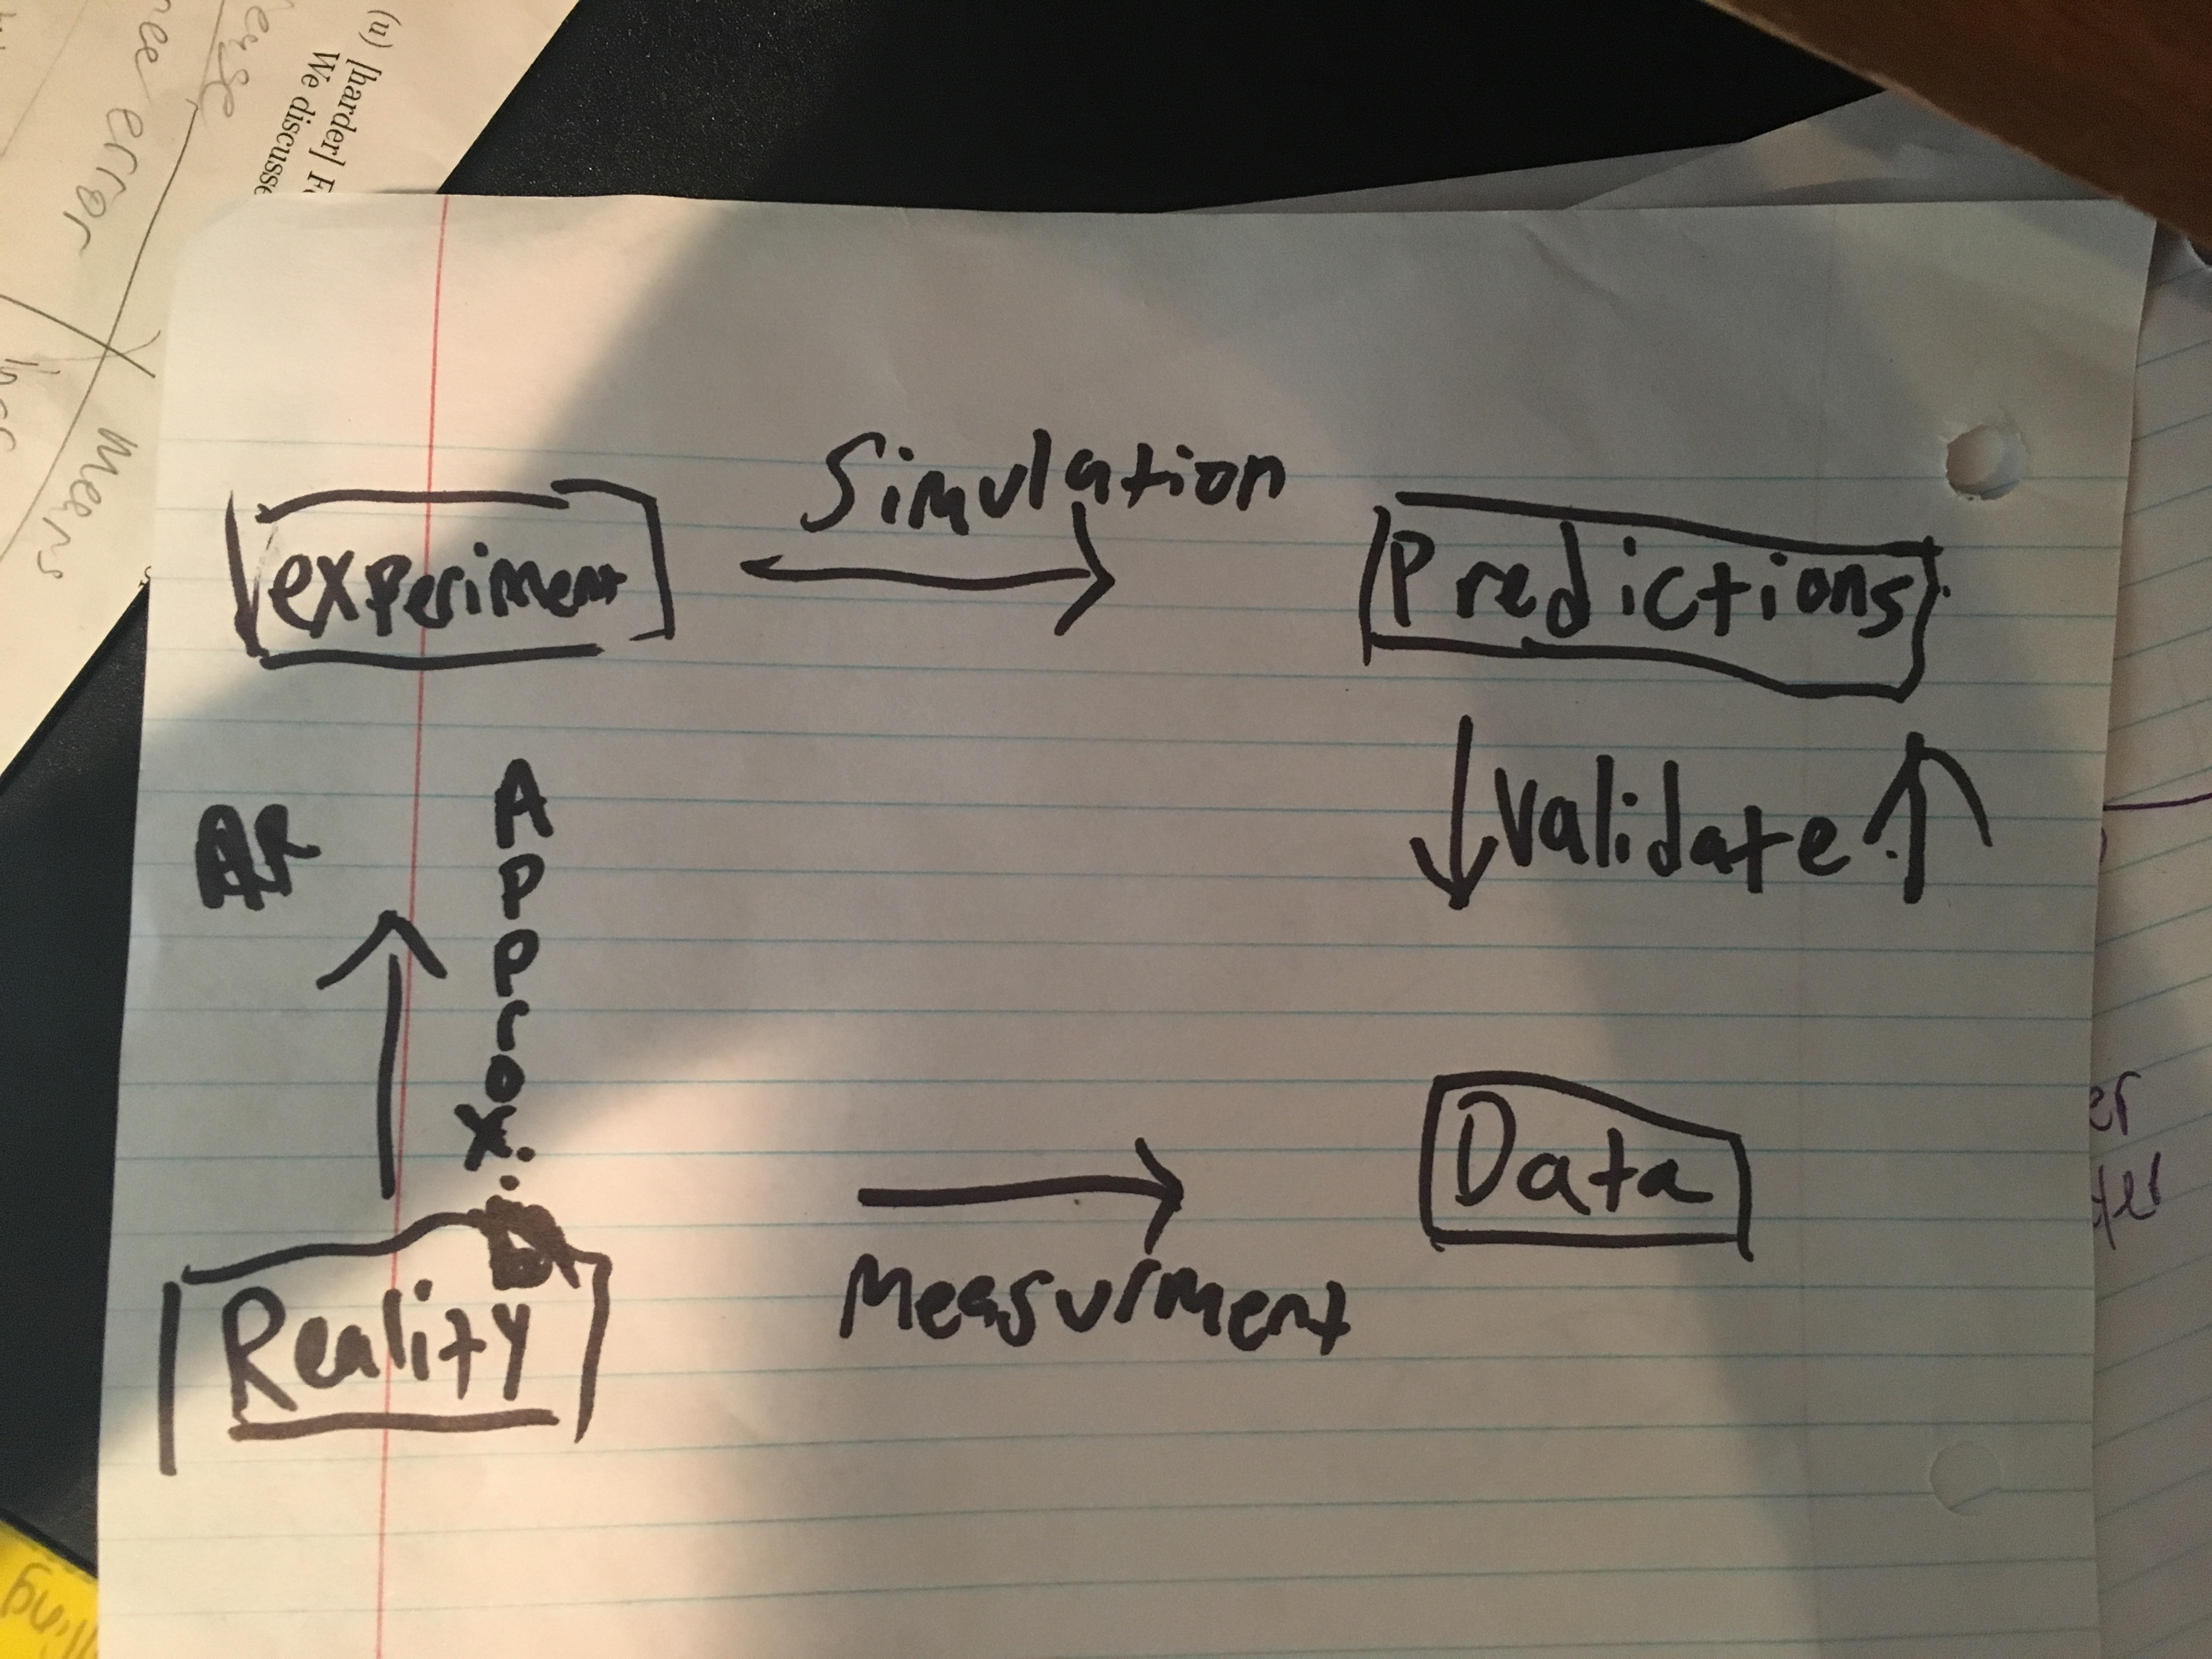
\includegraphics[width=3in]{hw1t_3a.jpg}
\end{figure}

\easysubproblem{Pursuant to the fix in the previous question, how do we define \emph{data} for the purposes of this class?}\spc{3}

Data is the measured response to a phenomenon.

\easysubproblem{Pursuant to the fix in the previous question, how do we define \emph{predictions} for the purposes of this class?}\spc{3}

Predictions are the response to the model we build $g$,

\easysubproblem{Why are \qu{all models wrong}? We are quoting the famous statisticians George Box and Norman Draper here.}\spc{2}

We can never know the "truth"

\intermediatesubproblem{Why are \qu{[some models] useful}? We are quoting the famous statisticians George Box and Norman Draper here.}\spc{2}

We can approximate the truth and derive useful results.

\easysubproblem{What is the difference between a "good model" and a "bad model"?}\spc{2}

When our predictions are close to the data we measured as the response to the phenomenon, we have a good model.
\end{enumerate}

\problem{We are now going to investigate the aphorism \qu{An apple a day keeps the doctor away}. We will use this as springboard to ask more questions about the framework of modeling we introduced in this class.}

\begin{enumerate}

\intermediatesubproblem{How good / bad do you think this model is and why?}\spc{3}

A bad model since it is extremely vague, like this answer.

\easysubproblem{Is this a mathematical model? Yes / no and why.}\spc{3}

Technically yes, since we could put it in mathematical terms.

\easysubproblem{What is(are) the input(s) in this model?}\spc{3}

If a person has eaten an apple in the last 24 hours(1) or not(0).

\easysubproblem{What is(are) the output(s) in this model?}\spc{3}
Either the doctor stays away(1) or he doesn't(0)
\easysubproblem{Devise a means to measure the main input. Call this $x_1$ going forward.}\spc{4}
Let $x_1$=apples eaten/24 hours
\easysubproblem{Devise a means to measure the main output. Call this $y$ going forward.}\spc{4}

Need to define a time period for the apple effect, see if person visited doctor during that amount of time following the eating of an apple

\easysubproblem{What is $\mathcal{Y}$ mathematically?}\spc{3}

$\mathcal{Y}\in\{0, 1\}$

\easysubproblem{Briefly describe $z_1, \ldots, z_t$ in English where $y = t(z_1, \ldots, z_t)$ in this \emph{phenomenon} (not \emph{model}).}\spc{3}

$\vec{z}$ are the unobservable aspects producing the phenomenon, for example the strength of a persons immune system. 

\easysubproblem{From this point on, you only observe $x_1$ is in the model. What is $p$ mathematically?}\spc{1}
 $p=1$

\intermediatesubproblem{From this point on, you only observe $x_1$ is in the model. What is $\mathcal{X}$ mathematically? If your information contained in $x_1$ is non-numeric, you must coerce it to be numeric at this point.}\spc{3}

$\mathcal{X}$=apples eaten/24 hours

\intermediatesubproblem{How did we term the functional relationship between $y$ and $x_1$?}\spc{3}
\begin{equation*}
y=f(x_1)
\end{equation*}

\easysubproblem{Briefly describe \emph{superivised learning}.}\spc{5}

Supervised learning is using historical records/responses to model a phenomenon. 

\easysubproblem{Why is \emph{superivised learning} a \emph{empirical solution} and not an \emph{analytic solution}?}\spc{3}

Supervised learning is not an analytical solution because there are no formulas to solve. We are using the data to create an answer, hence empirical.

\intermediatesubproblem{From this point on, assume we are involved in supervised learning to achieve the goal you stated in the previous question. Briefly describe what $\mathbb{D}$ would look like here.}\spc{3}
\begin{equation*}
\mathbb{D}=\{<x_1, y_1>, \cdots, <x_n, y_n>\}
\end{equation*}
Each $<x_i, y_i>$ represents how many apples a person ate in 24 hours and whether or not the same person visited the doctor within a specific amount of time following their apple consummation. 
\intermediatesubproblem{Briefly describe the role of $\mathcal{H}, \mathcal{A}$ here.}\spc{3}

$\mathcal{H}$ is the set of all candidate functions that approximate the phenomenom we are trying model. $\mathcal{A}$ takes in $\mathbb{D}, \mathcal{H}$ and returns the "best" choice in $\mathcal{H}$.

\easysubproblem{If $g = \mathcal{A}(\mathbb{D}, \mathcal{H})$, what should the domain and range of $g$ be?}\spc{3}

The domain of $g$ would be all $\mathbb{R}$ and the range would be ${0,1}$

\easysubproblem{Is $g \in \mathcal{H}$? Why or why not?}\spc{3}

Yes, $g \in \mathcal{H}$. $\mathcal{A}$ returns a function from $\mathcal{H}$ and since $g=\mathcal{A}(\mathbb{D}, \mathcal{H})$, $g$ must be an element in $\mathcal{H}$

\easysubproblem{Given a never-before-seen value of $x_1$ which we denote $x^*$, what formula would we use to predict the corresponding value of the output? Denote this prediction $\hat{y}^*$.}\spc{3}
\begin{equation*}
\hat{y}^*=g(x^*)
\end{equation*}

\intermediatesubproblem{Is it reasonable to assume $f \in \mathcal{H}$? Why or why not?}\spc{4}

No it is not reasonable because we don't even know what $f$ is. 

\easysubproblem{If $f \notin \mathcal{H}$, what are the three sources of error? Write their names and provide a sentence explanation of each. Note that I made a notational mistake in the notes based on what is canonical in data science. The difference $t - g$ should be termed $e$ as the term $\mathcal{E}$ is reserved for $t - h^*$.}\spc{4}

\begin{enumerate}
\item Parameter Estimation Error $h^*(\vec{x})-g(\vec{x})$: we don't always pick the best candidate model from the set.
\item Misspecification Error $f(\vec{x})-h^*(\vec{x})$ $f \notin \mathcal{H}$, if $f$ is a curve and we choose $\mathcal{H}$ to be lines, $h^*$ is going to differ from $f$.
\item Ignorance Error $t(\vec{x})-f(\vec{x})$ we can never know the truth.
\end{enumerate}

\intermediatesubproblem{For each of the three source of error, provide a means of reducing the error. We discussed this in class.}\spc{4}

\begin{enumerate}
\item Parameter estimation error can be decreased with a larger $n$
\item Misspecification Error can be decreased by a better $\mathcal{A}$
\item Ignorance Error can be decreased by adding features $p$.
\end{enumerate}

\easysubproblem{Regardless of your answer to what $\mathcal{Y}$ was above, we now coerce $\mathcal{Y} = \braces{0,1}$. If we use a threshold model, what would $\mathcal{H}$ be? What would the parameter(s) be?}\spc{3}

\begin{equation*}
\mathcal{H}=\{\mathbb{I}_{x\geq x_T}\}
\end{equation*}
The parameters of $\mathcal{H}$ are $x_T$.

\easysubproblem{Give an explicit example of $g$ under the threshold model.}\spc{3}
\begin{equation*}
g(\vec{x})=\mathbb{I}_{x\geq1}
\end{equation*}
\end{enumerate}

\problem{These are questions about the linear perceptron. This problem is not related to problem 3.}

\begin{enumerate}

\easysubproblem{For the linear perceptron model and the linear support vector machine model, what is $\mathcal{H}$? Use $b$ as the bias term.}\spc{3}

\begin{equation*}
\mathcal{H}=\{\mathbb{I}_{b\cdot\vec{x}>0}\:\vec{b}\in\mathbb{R}^{p+1}\}
\end{equation*}

\intermediatesubproblem{Rewrite the steps of the \emph{perceptron learning algorithm} using $b$ as the bias term.}\spc{13}

\begin{enumerate}
\item Initiate the weights to be $\vec{b}=0$ or random
\item Calculate $\yhat_i=\mathbb{I}_{b_0\cdot\vec{x_i}>0}$
\item update all weights $j=0,\cdots, p$ \begin{eqnarray*}
b_0^{t=1}=b_0^{t=0}+(y_i-\hat{y_i}) &&  (1)\\
b_1^{t=1}=b_1^{t=0}+(y_i-\hat{y_i}) && (x_{i,1})\\
\vdots \\
b_p^{t=1}=b_p^{t=0}+(y_i-\hat{y_i}) && (x_i,p)
\end{eqnarray*}
\item Repeat steps (b) and (c) $\forall i\in\{1,\cdots, n\}$
\item Repeat setps (b)-(d) until error hits threshold or a prespecfied number of iterations are run.
\end{enumerate}

\easysubproblem{Illustrate the perceptron as a one-layer neural network with the Heaviside / binary step / indicator function activation function.}\spc{10}

\begin{figure}[htp]
\centering
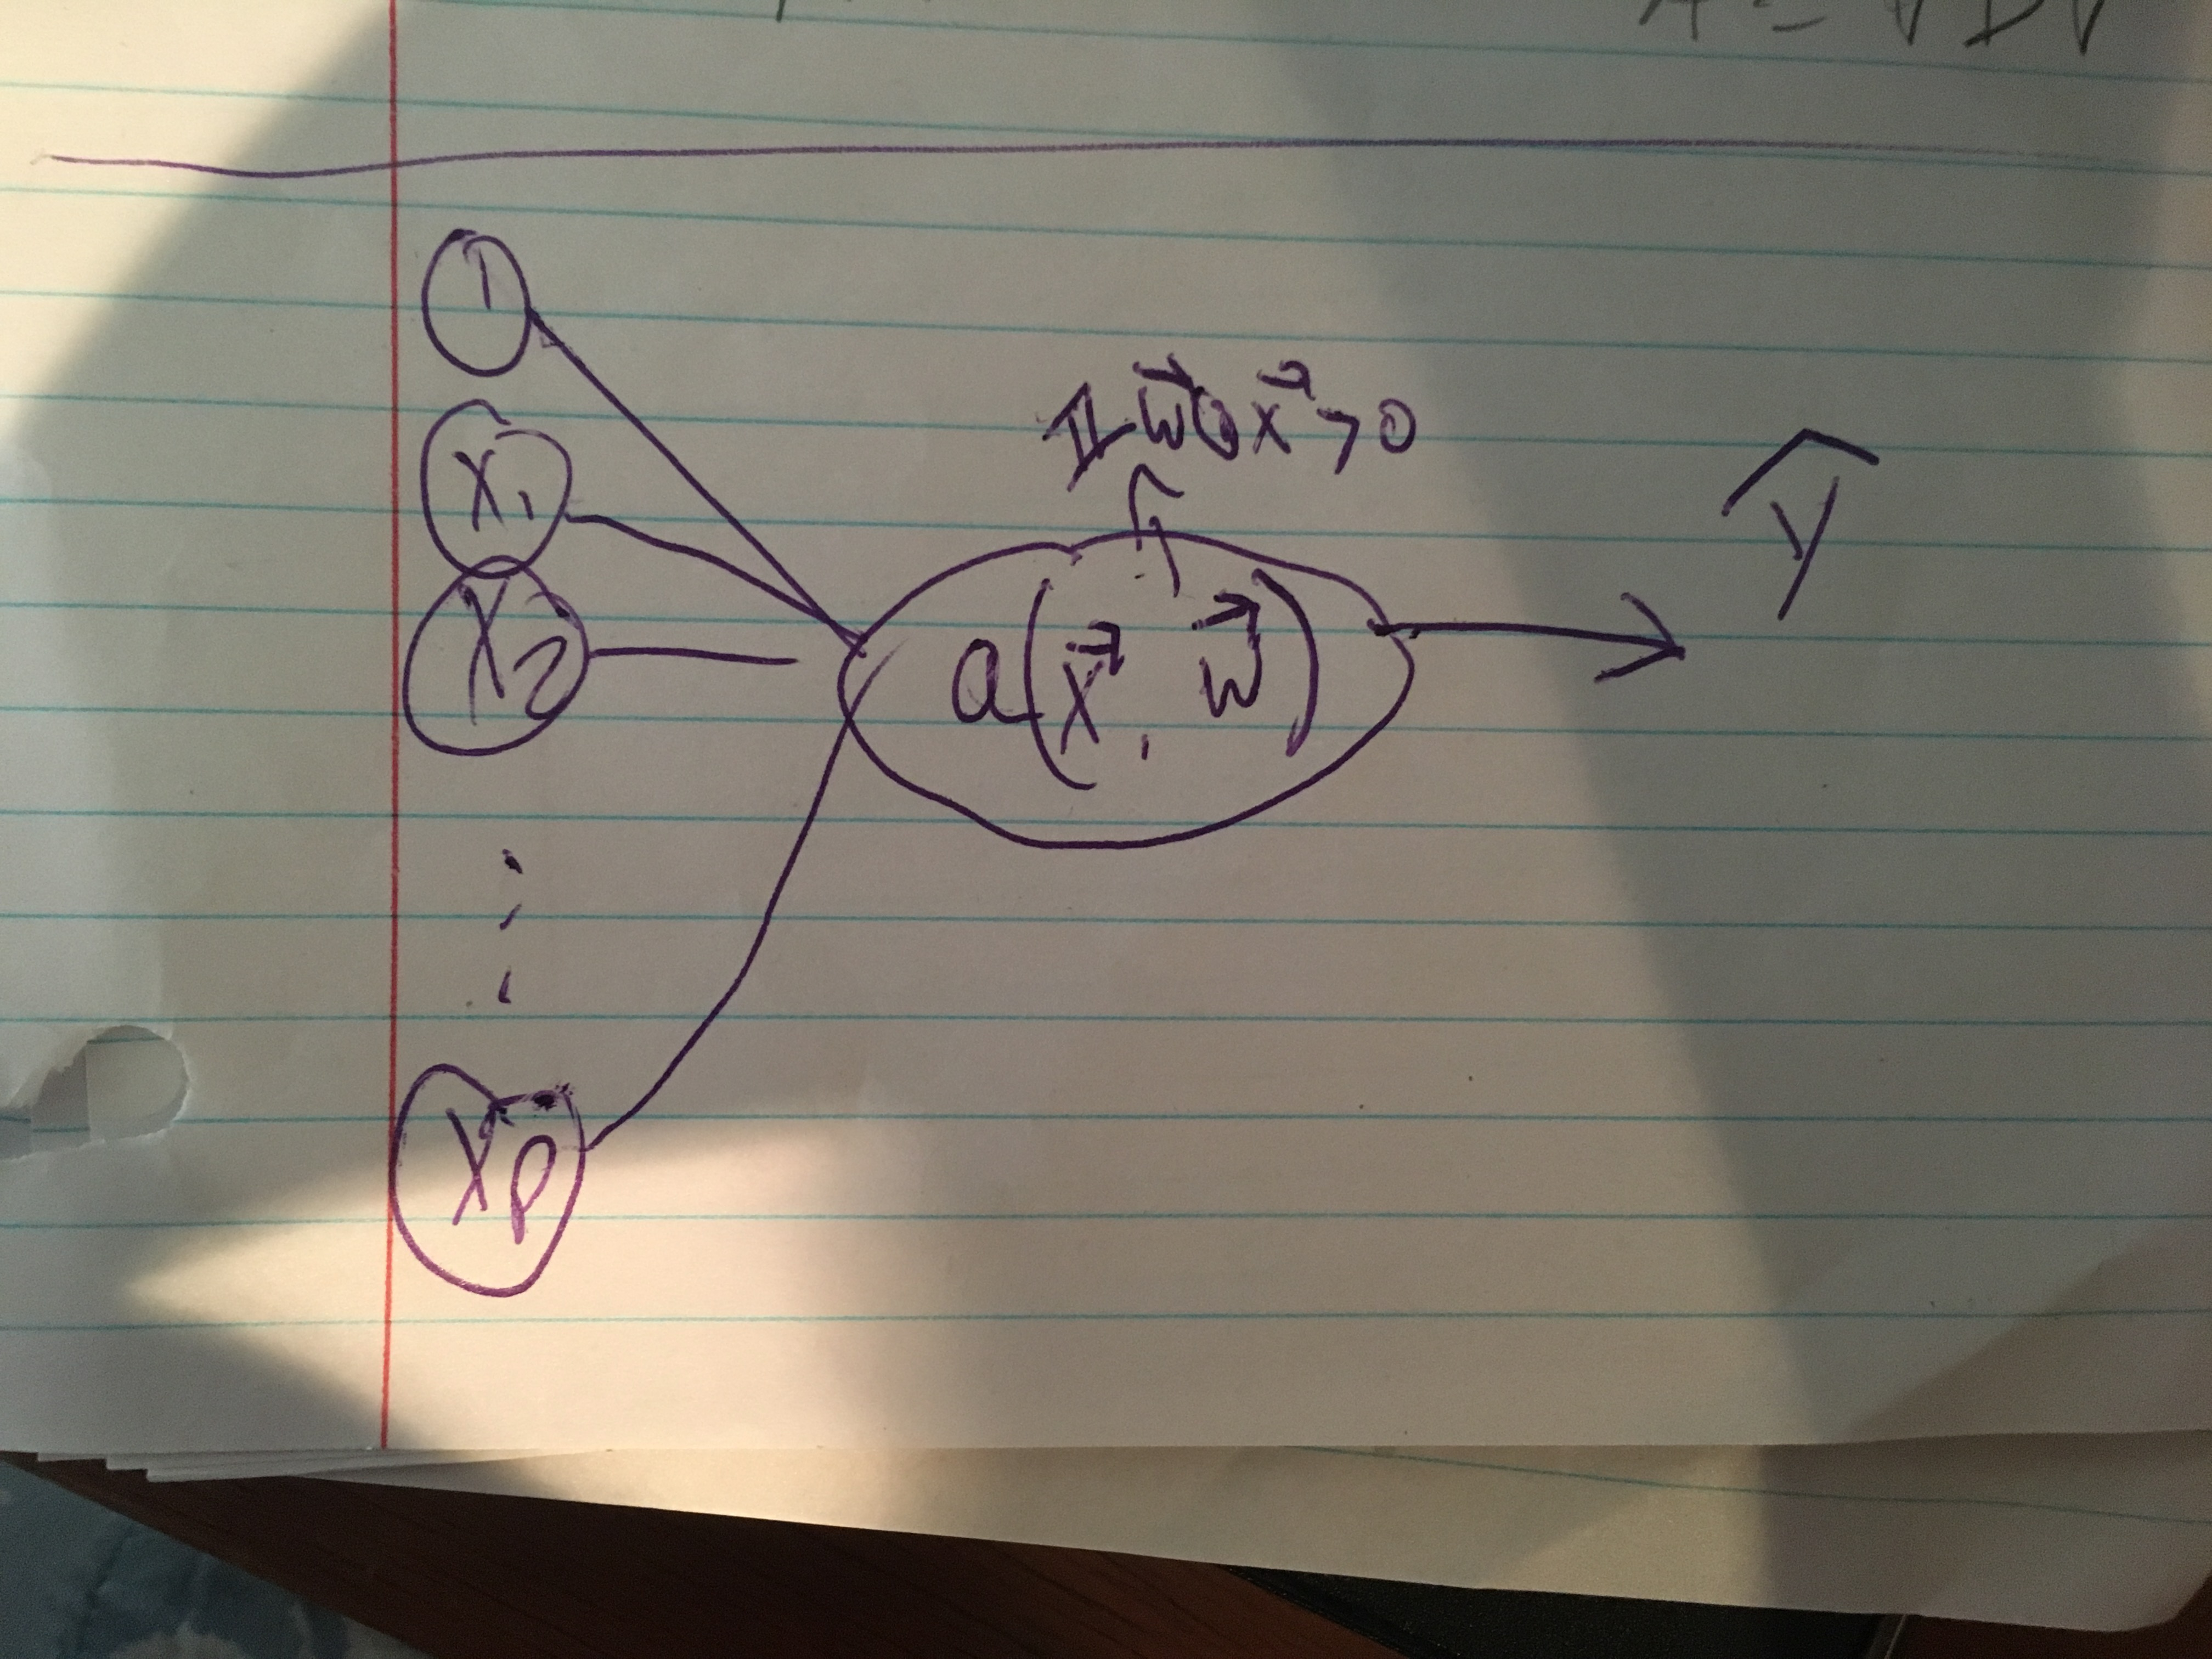
\includegraphics[width=3in]{hw1t_4c.jpg}
\end{figure}

\easysubproblem{Provide an illustration of a two-layer neural network. Be careful to indicate all pieces. If a mathematical object has a different value from another mathematical object, denote it differently.}\spc{10}

\begin{figure}[htp]
\centering
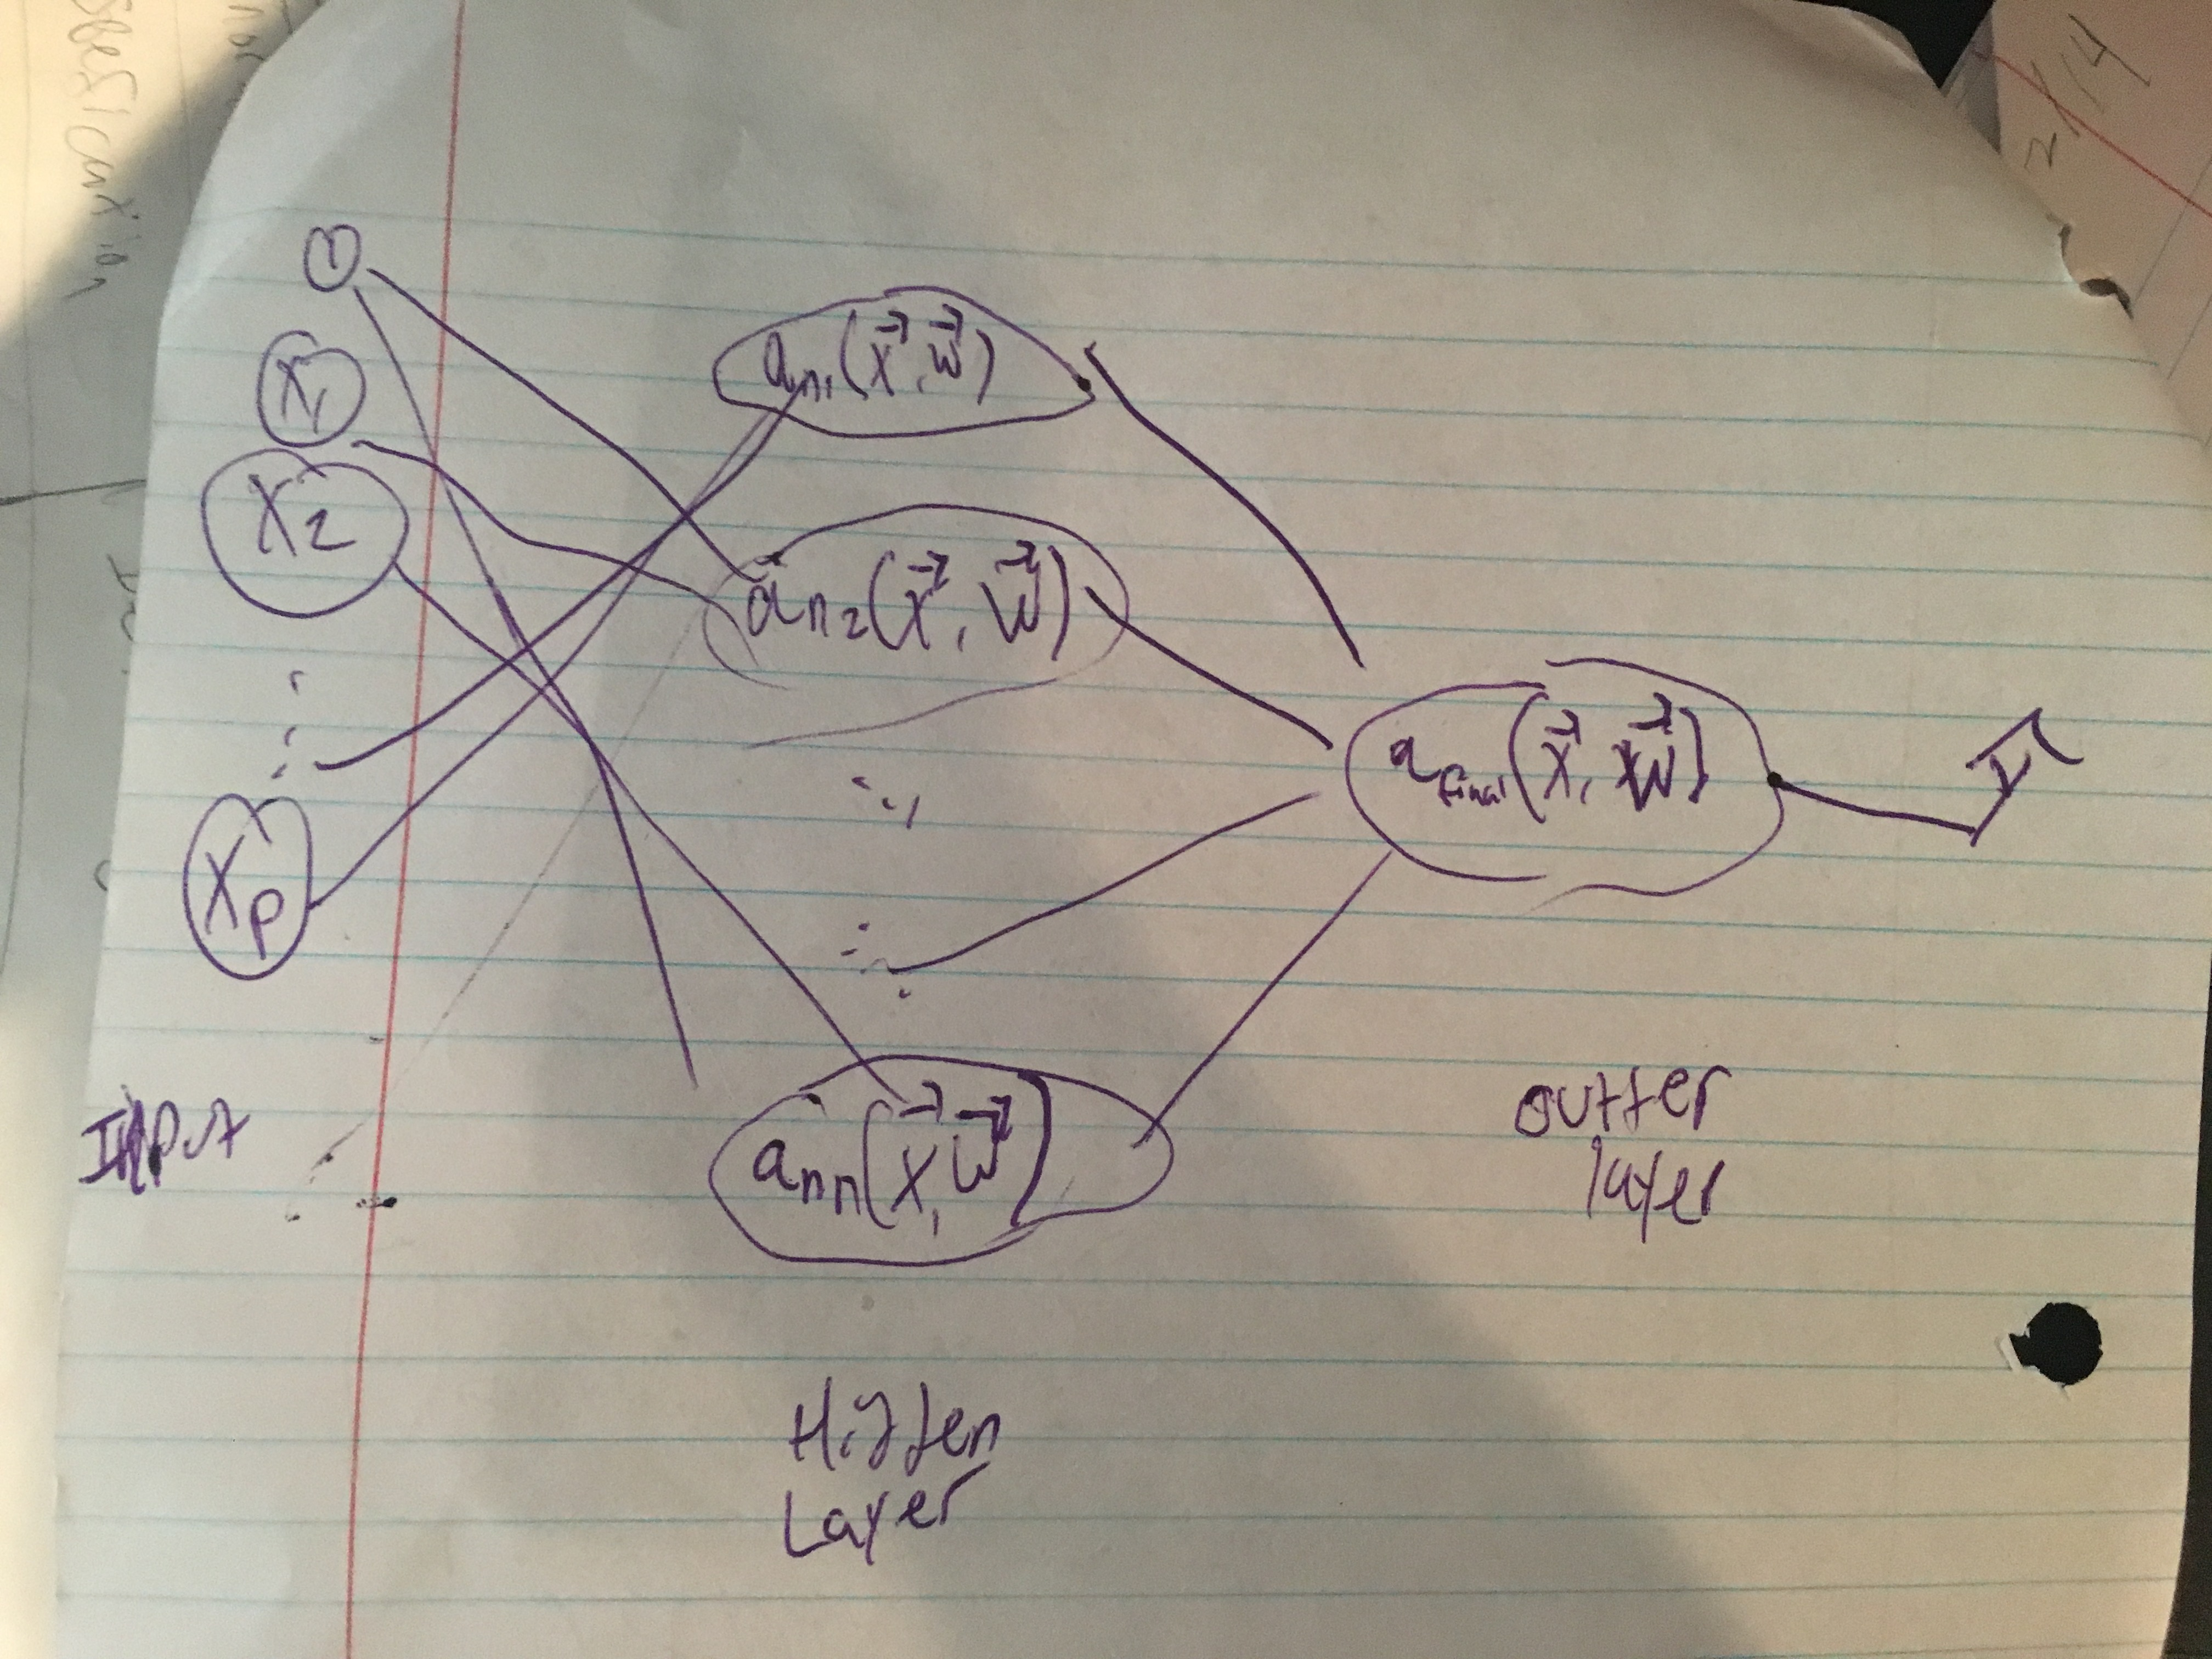
\includegraphics[width=2in]{hw1t_4d.jpg}
\end{figure}
\end{enumerate}

\end{document}











%Why was it such a bad idea for the rating agencies to allow their clients to use their formula?
%Explain the different between foxes and hedgehogs

\problem{These are questions about Silver's book, introduction, chapter 1, 2 and 3.}

\begin{enumerate}

\easysubproblem{Explain Hume's problem of induction with the sun rising every day.}\spc{3}

\easysubproblem{Explain the \qu{inverse probability problem.}}\spc{3}

\easysubproblem{What is Bayes' billiard table problem?}\spc{3}

\hardsubproblem{[MA] How did Price use Bayes' idea to prove the existence of the deity?} \spc{3}

\easysubproblem{Why should Bayes Rule really be called \qu{Laplace's Rule?}}\spc{3}

\hardsubproblem{Prove the version of Bayes Rule found on page 20. State your assumption(s) explicitly. Reference class notes as well.}\spc{4}

\easysubproblem{Give two scientific contexts where Laplace used inverse probability theory to solve major problems.}\spc{3}

\hardsubproblem{[MA] Why did Laplace turn into a frequentist later in life?} \spc{3}

\easysubproblem{State Laplace's version of Bayes Rule (p31).} \spc{3}

\easysubproblem{Why was Bayes Rule \qu{damned} (pp36-37)?} \spc{3}

\easysubproblem{According to Edward Molina, what is the prior (p41)?} \spc{3}

\easysubproblem{What is the source of the \qu{credibility} metric that insurance companies used in the 1920's?} \spc{3}

\easysubproblem{Can the principle of inverse probability work without priors? Yes/no.} \spc{1}

\hardsubproblem{In class we discussed the \qu{principle of indifference} which is a term I borrowed from \href{http://www.amazon.com/Philosophical-Theories-Probability-Issues-Science/dp/041518276X/ref=sr_1_1?ie=UTF8&qid=1455112335&sr=8-1&keywords=donald+gillies+theory+of+probability}{Donald Gillies' Philosophical Theories of Probability}. On Wikipedia, it says that Jacob Bernoulli called it the \qu{principle of insufficient reason}. McGrayne in her research of original sources comes up with many names throughout history this principle was named. List all of them you can find here.} \spc{3}

\easysubproblem{Jeffreys seems to be the founding father of modern Bayesian Statistics. But why did the world turn frequentist in the 1920's? (p57)} \spc{3}
\end{enumerate}

\problem{These exercises will review the Bernoulli model.}


\begin{enumerate}

\easysubproblem{If $X \sim \bernoulli{\theta}$, find $\expe{X}$, $\var{X}$, $\support{X}$ and $\Theta$. No need to derive from first principles, just find the formulas.}\spc{2}

\intermediatesubproblem{If $X \sim \bernoulli{\theta}$, find $\median{X}$.}\spc{2}

\intermediatesubproblem{If $X \sim \bernoulli{\theta}$, write the \qu{parametric statistical model} below using the notation we used in class only.}\spc{2}


\intermediatesubproblem{Explain what the semicolon notation in the previous answer indicates. Hint: go back to precalc and think of the function $g(x;a) = ax^2$ }\spc{2}

\easysubproblem{If $\Xoneton \iid \bernoulli{\theta}$, find the likelihood, $\mathcal{L}$, of $\theta$.}\spc{2}

\hardsubproblem{Given the likelihood above, what would $\mathcal{L}$ be if the data was $<0,1,0,1,3.7>$? Why should this answer have to be?}\spc{2}

\easysubproblem{If $\Xoneton \iid \bernoulli{\theta}$, find the log-likelihood of $\theta$, $\ell(\theta)$.}\spc{2}

\hardsubproblem{[MA] If $\Xoneton \iid f(x;\theta)$, explain why the log-likelihood of $\theta$ is normally distributed if $n$ gets large.}\spc{6}

\easysubproblem{If $\Xoneton \iid \bernoulli{\theta}$, find the score function (i.e the derivative of the log-likelihood) of $\theta$.}\spc{2}

\intermediatesubproblem{If $\Xoneton \iid \bernoulli{\theta}$, find the maximum likelihood estimator for $\theta$.}\spc{5}

\easysubproblem{If $\Xoneton \iid \bernoulli{\theta}$, find the maximum likelihood \textit{estimate} for $\theta$.}\spc{1}

\easysubproblem{Given the previous two questions, describe the difference between a random variable and a datum.}\spc{3}

\easysubproblem{If your data is $<0,1,1,0,1,1,0,1,1,1>$, find the maximum likelihood estimate for $\theta$.}\spc{1}

\easysubproblem{Given this data, find a 99\% confidence interval for $\theta$.}\spc{3}

\easysubproblem{Given this data, test $H_0: \theta = 0.5$ versus $H_a: \theta \neq 0.5$.}\spc{7}


\easysubproblem{Write the PDF of $X \sim \normnot{\theta}{1^2}$.}\spc{5}

\hardsubproblem{Find the MLE for $\theta$ if $\Xoneton \iid \normnot{\theta}{1^2}$.}\spc{6}

\hardsubproblem{[MA] Find the MLE for $\theta$ if $\Xoneton \iid \normnot{\mu}{\sigsq}$. Solve the system of equations $\partialop{\mu}{\ell(\theta)} = 0$ and $\partialop{\sigsq}{\ell(\theta)} = 0$ where $\ell(\theta)$ denotes the log likelihood. You can easily find this online. But try to do it yourself.} \spc{20}


\end{enumerate}

\problem{We will review the frequentist perspective here.}

\begin{enumerate}

\hardsubproblem{Why do frequentists have an insistence on $\theta$ being a fixed, immutable quantity? We didn't cover this in class explicitly but it is lurking behind the scenes. Use your reference resources.}\spc{5}

\easysubproblem{What are the three goals of inference? Give short explanations.}\spc{5}

\easysubproblem{What are the three reasons why \emph{frequentists} (adherents to the frequentist perspective) use MLEs i.e. list three properties of MLEs that make them powerful.}\spc{6}

\hardsubproblem{[MA] Give the conditions for asymptotic normality of the MLE,

\beqn
\frac{\thetahatmle - \theta}{\se{\thetahatmle}} \convd \stdnormnot.
\eeqn

You can find them online.}\spc{8}

\hardsubproblem{[MA] $\se{\thetahatmle}$ cannot be found without $\theta$ so we substituted $\thetahatmle$ into $\se{\thetahatmle}$ and called it $\seest{\thetahatmle}$ (note the hat over the SE). Show that this too is asymptotically normal, \ie

\beqn
\frac{\thetahatmle - \theta}{\seest{\thetahatmle}} \convd \stdnormnot
\eeqn

You need the continuous mapping theorem and Slutsky's theorem.
}\spc{4}

\easysubproblem{[MA] Explain why the previous question allows us to build asymptotically valid confidence intervals using $\bracks{\thetahatmle \pm z_{\alpha/2} \seest{\thetahatmle}}$}.\spc{3}

\intermediatesubproblem{Why does all of frequentist inference break down if $n$ isn't large?}\spc{2}

\easysubproblem{Write the most popular two frequentist interpretations of a confidence interval.}\spc{6}

\intermediatesubproblem{Why are each of these unsatisfactory?}\spc{3}

\easysubproblem{What are the two possible outcomes of a hypothesis test?}\spc{1}

\hardsubproblem{[MA] What is the weakness of the interpretation of the $p$-val?}\spc{6}


\end{enumerate}


\problem{We review and build upon conditional probability here.}

\begin{enumerate}


\easysubproblem{Explain why $\cprob{B}{A} \propto \cprob{A}{B}$.}\spc{6}

\easysubproblem{If $B$ represents the hypothesis or the putative cause and $A$ represents evidence or data, explain what Bayesian Conditionalism is, going from which probability statement to which probability statement.}\spc{3}

\end{enumerate}


\end{document}








%%%%%%%%%%%%%%%%%%%%%%%%%%%%%%%%%%%%%%%%



\intermediatesubproblem{In class we presented the posterior odds form of Bayes Theorem. Prove it below.}\spc{10}


\intermediatesubproblem{Show that the Bayes Factor is the ratio of posterior odds of the hypothesis to prior odds of the hypothesis.}\spc{2}

\easysubproblem{On the \href{https://en.wikipedia.org/wiki/Bayes_factor}{wikipedia page about Bayes Factors}, Harrold Jeffreys (who we will be returning to later in the semester) gave interpretations of Bayes Factors (which is denoted $K$ there and $B$ in Bolstad's book on page 70). Give the ranges of $K$ here (not in terms of powers of 10, but as a pure number) for his interpretations i.e. \qu{negative,} \qu{strong,} etc.}\spc{3}

\hardsubproblem{[MA] Conceptually why should the likelihood being greater than $\prob{A}$ imply that the hypothesis is more likely after observing the data than before?}\spc{6}
\end{enumerate}

\problem{We examine here paternity testing (i.e. answering the question \qu{is this guy the father of my child?}) via the simplistic test using blood types. These days, more advanced genetic methods exist so these calculations aren't made in practice, but they are a nice exercise. 

First a crash course on basic genetics. In general, everyone has two alleles (your genotype) with one coming from your mother and one coming from your father. The mother passes on each of the alleles with 50\% probability and the father passes on each allele with 50\% probability. One allele gets expressed (your phenotype). So one of the genes shone through (the dominant one) and one was masked (the recessive one). Dominant blood types are A and B and the recessive type is o (lowercase letter). The only way to express phenotype o is to have genotype oo i.e. both genes are o. There is an exception; A and B are codominant meaning that blood type AB tests positive for both A and B.

In this case consider a child of blood type B and the mother of blood type A. Using this \href{http://www.cccoe.net/genetics/blood2.html}{hereditary guide}, we know that the mother's type must be Ao so she passed on an o to the child thus the child got the B from the father. Thus the father had type AB, BB or Bo. I got the following data from \href{http://www.sciencedirect.com/science/article/pii/S1110863011000796}{this paper} (so let's assume this case is in Nigeria in 1998).

\begin{table}
\centering
\begin{tabular}{cc}
Genotype & Frequency \\ \hline
OO	&0.52 \\
AA	&0.0196 \\
AO	&0.2016 \\
BB	&0.0196 \\
BO	&0.2016 \\
AB	&0.0392 \\
\end{tabular}
\end{table}
} 

\begin{enumerate}

\easysubproblem{Bob is the alleged father and he has blood type B but his genotype is unknown. What is the probability he passes on a B to the child?}\spc{3}

\easysubproblem{What is the probability a stranger passes on a B to the child?}\spc{3}

\easysubproblem{Assume our prior is 50-50 Bob is the father, the customary compromise between a possibly bitter mother and father. What is the prior odds of Bob being the father? Don't think too hard about this one; it is marked easy for a reason.}\spc{6}

\hardsubproblem{We are interested in the posterior question. What is the probability Bob is the father given the child with blood type B?}\spc{5}

\hardsubproblem{What is the Bayes Factor here? See (a) and (b).}\spc{5}

\easysubproblem{What is the probability Bob is not the father given the child with blood type B? Should be easy once you have (c) and (e).}\spc{3}

\end{enumerate}


\end{document}
